
%=======================================================================
\chapter{Introduction}
\label{ch:intro}

\textbf{%
This chapter is \emph{frozen} and has already passed public review,
making a functional change at this stage extremely unlikely.%
}
\bigskip

This document specifies the Advanced Interrupt Architecture for
{\RISCV}, consisting of:
(a)~an extension to the standard Privileged Architecture for {\RISCV}
harts specified in Volume~II of The {\RISCV} Instruction Set Manual;
(b)~two standard interrupt controllers for {\RISCV} systems, an
Advanced Platform-Level Interrupt Controller (APLIC) and an
Incoming Message-Signaled Interrupt Controller (IMSIC); and
(c)~requirements on other system components concerning interrupts.

\begin{commentary}
Commentary on our design decisions, implementation options, and
application is formatted as in this paragraph, and can be skipped if
the reader is only interested in the specification itself.
\end{commentary}

%-----------------------------------------------------------------------
\section{Goals}

The {\RISCV} Advanced Interrupt Architecture has these goals:
\begin{itemize}

\item
Build upon the interrupt-handling functionality of the {\RISCV}
Privileged Architecture, minimizing the replacement of existing
functionality.

\item
Provide facilities for {\RISCV} systems to work directly with
message-signaled interrupts (MSIs) as employed by PCI Express and other
device standards, in addition to basic wired interrupts.

\item
For wired interrupts, define a new Platform-Level Interrupt Controller
(the Advanced PLIC, or APLIC)
that has an independent control interface for each
level of privilege (such as {\RISCV} machine and supervisor levels),
and that can convert wired interrupts into MSIs for systems supporting
MSIs.

\item
Expand the framework for local interrupts at a {\RISCV} hart.

\item
Optionally allow software to configure the relative priorities of all
sources of interrupts to a {\RISCV} hart (including the standard timer
and software interrupts, among others), instead of being limited
just to the ability of a separate interrupt controller to prioritize
external interrupts only.

\item
When harts implement the Privileged Architecture's hypervisor
extension, provide sufficient assistance for virtualizing these same
interrupt facilities for virtual machines.

\item
With the help of an \mbox{IOMMU} (I/O memory management unit) for redirecting
MSIs, maximize the opportunities and ability for a guest operating
system running in a virtual machine to have direct control of devices
with minimal involvement of a hypervisor.

\item
Avoid having the interrupt hardware be a limiter on the number of
virtual machines.

\item
Achieve all of the above with the best possible compromises between
speed, efficiency, and flexibility of implementation.

\end{itemize}

This initial version of the Advanced Interrupt Architecture is focused
primarily on the needs of larger, high-performance {\RISCV} systems.
Support is not currently defined for the following interrupt-handling
features that are useful for minimizing interrupt response times in
so-called ``real-time'' systems but are less appropriate for high-speed
processor cores:
\begin{tightList}
\item
the option to give each interrupt source at a hart a separate trap
entry address;
\item
automatic stacking of register values on interrupt trap entry, and
restoration on exit; and
\item
automatic preemption (nesting) of interrupts at a hart, based on
priority.
\end{tightList}
It is intended that such features optimizing for smaller and/or
real-time systems can be developed as a follow-on extension, either
separately or as part of a future version of the interrupt architecture
of this document.

%-----------------------------------------------------------------------
\section{Limits}

In its current version, the {\RISCV} Advanced Interrupt Architecture
can support {\RISCV} symmetric multiprocessing (SMP) systems with up to
16,384 harts.
If the harts are \mbox{64-bit} (RV64) and implement the hypervisor
extension, and if all features of the Advanced Interrupt Architecture
are fully implemented as well, then for each physical hart there may be
up to 63 active virtual harts and potentially thousands of additional
idle (swapped-out) virtual harts, where each virtual hart has direct
control of one or more physical devices.

Table~\ref{tab:overallLimits} summarizes the main limits on the numbers
of harts, both physical and virtual, and the numbers of distinct
interrupt identities that may be supported with the Advanced Interrupt
Architecture.

\begin{table*}[h!]
\begin{center}
\begin{tabular}{|l|c|l|}
\hline
   & Maximum      & \multicolumn{1}{c|}{Requirements} \\
\hline
\hline
Physical harts
   & 16,384       & \\
\hline
Active virtual harts having direct control of \quad
   & 31 for RV32, & {\RISCV} hypervisor extension; \\
\ a device, per physical hart
   & 63 for RV64  & \ IMSICs with guest interrupt\\
   &              & \ files; and an IOMMU \\
\hline
Idle (swapped-out) virtual harts having \quad
   & potentially  & An IOMMU with support \\
\ direct control of a device, per physical hart \quad
   & thousands    & \ for memory-resident \\
   &              & \ interrupt files \\
\hline
Wired interrupts at a single APLIC \quad
   & 1023         & \\
\hline
Distinct identities usable for MSIs at each \quad
   & 2047         & IMSICs \\
\ hart (physical or virtual)
   &              & \\
\hline
\end{tabular}
\end{center}
\caption{%
Absolute limits on the numbers of harts and interrupt identities in a
system.
Individual implementations are likely to have smaller limits.%
}
\label{tab:overallLimits}
\end{table*}

\begin{commentary}
We assume that any single {\RISCV} computer (or any single node in a
cluster or distributed system) with many thousands of physical harts
will probably need an interrupt infrastructure adapted to the machine's
specific organization, which we do not attempt to predict.
\end{commentary}

%-----------------------------------------------------------------------
\section{Overview of main components}

A {\RISCV} system's overall architecture for signaling interrupts
depends on whether it is built mainly for message-signaled interrupts
(MSIs) or for more traditional wired interrupts.
In systems with full support for MSIs, every hart has an
\emph{Incoming MSI Controller} (IMSIC) that serves as the hart's own
private interrupt controller for external interrupts.
Conversely, in systems based primarily on traditional wired interrupts,
harts do not have IMSICs.
Larger systems, and especially those with PCI devices, are
expected to fully support MSIs by giving harts IMSICs, whereas many
smaller systems may continue to be best served with wired interrupts
and simpler harts without IMSICs.

%- - - - - - - - - - - - - - - - - - - - - - - - - - - - - - - - - - - -
\subsection{External interrupts without IMSICs}

When {\RISCV} harts do not have Incoming MSI Controllers, external
interrupts are signaled to harts through dedicated wires.
In that case, an \emph{Advanced Platform-Level Interrupt Controller}
(APLIC) acts as a traditional central hub for interrupts,
routing and prioritizing external interrupts for each hart as
illustrated in Figure~\ref{fig:intrsWithoutIMSICs}.
Interrupts may be selectively routed either to machine level or to
supervisor level at each hart.
The APLIC is specified in Chapter~\ref{ch:AdvPLIC}.

\begin{figure}[th]
\centerline{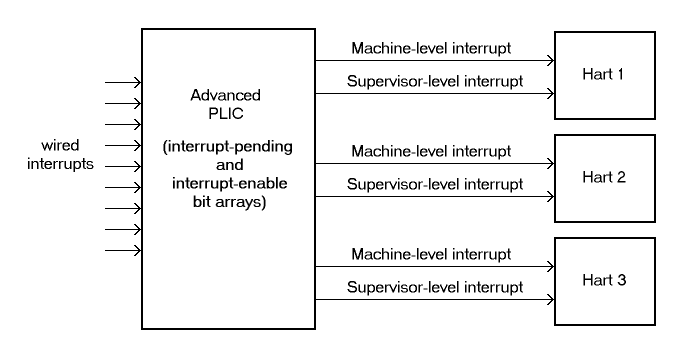
\includegraphics[scale=0.55]{intrsWithoutIMSICs.png}}
\caption{%
Traditional delivery of wired interrupts to harts without support for
MSIs.%
}
\label{fig:intrsWithoutIMSICs}
\end{figure}

Without IMSICs, the current Advanced Interrupt Architecture does
not support the direct signaling of external interrupts to virtual
machines, even when {\RISCV} harts implement the Privileged
Architecture's hypervisor extension.
Instead, an interrupt must be sent to the relevant hypervisor, which
can then choose to inject a virtual interrupt into the virtual machine.

\begin{commentary}
If harts implement the hypervisor extension, it is a topic of ongoing
study whether an APLIC should be allowed to route external
interrupts to be the \emph{guest external interrupts} of the hypervisor
extension, permitting the delivery of interrupts directly to virtual
machines without the need for each signaled interrupt to be handled at
the hypervisor level.
For now, we assume that systems that need direct signaling of external
interrupts to virtual machines will have IMSICs.
\end{commentary}

\begin{figure}[th]
\centerline{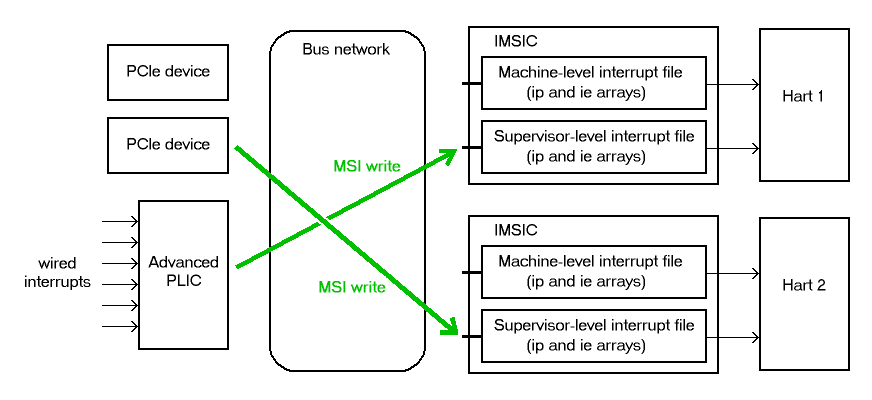
\includegraphics[scale=0.55]{intrsWithIMSICs.png}}
\caption{%
Interrupt delivery by MSIs when harts have IMSICs for receiving them.%
}
\label{fig:intrsWithIMSICs}
\end{figure}

%*** REMOVE?:
\FloatBarrier

%- - - - - - - - - - - - - - - - - - - - - - - - - - - - - - - - - - - -
\subsection{External interrupts with IMSICs}

To be able to receive message-signaled interrupts (MSIs), each
{\RISCV} hart must have an Incoming MSI Controller (IMSIC) as shown in
Figure~\ref{fig:intrsWithIMSICs}.
Fundamentally, a message-signaled interrupt is simply a memory write to
a specific address that hardware accepts as indicating an interrupt.
To that end, every IMSIC is assigned one or more distinct addresses in
the machine's address space, and when a write is made to one of those
addresses in the expected format, the receiving IMSIC interprets the
write as an external interrupt for the respective hart.

Because all IMSICs have unique addresses in the machine's physical
address space, every IMSIC can receive MSI writes from any agent (hart
or device) with permission to write to it.
IMSICs have separate addresses for MSIs directed to machine and
supervisor levels, in part so the ability to signal interrupts at each
privilege level can be separately granted or denied by controlling
write permissions at the different addresses, and in part to better
support virtualizability (pretending that one privilege level is a
higher level).
MSIs intended for a hart at a specific privilege level are recorded
within the IMSIC in an \emph{interrupt file}, which consists mainly
of an array of interrupt-pending bits and a matching array of
interrupt-enable bits, the latter indicating which individual
interrupts the hart is currently prepared to receive.

IMSIC units are fully defined in Chapter~\ref{ch:IMSIC}.
The format of MSIs used by the {\RISCV} Advanced Interrupt Architecture
is described in that chapter, Section~\ref{sec:MSIEncoding}.

When the harts in a {\RISCV} system have IMSICs, the system will
normally still contain an APLIC, but its role is changed.
Instead of signaling interrupts to harts directly by wires as in
Figure~\ref{fig:intrsWithoutIMSICs}, an APLIC converts incoming
wired interrupts into MSI writes that are sent to harts via their IMSIC
units.
Each MSI is sent to a single target hart according to the APLIC's
configuration set by software.

If {\RISCV} harts implement the Privileged Architecture's hypervisor
extension, IMSICs may have additional \emph{guest interrupt files} for
delivering interrupts to virtual machines.
Besides Chapter~\ref{ch:IMSIC} on the IMSIC, see
Chapter~\ref{ch:VSLevel} which specifically covers interrupts to
virtual machines.
If the system also contains an \mbox{IOMMU} to perform address translation
of memory accesses made by I/O devices, then MSIs from those same
devices may require special handling.
This topic is addressed in Chapter~\ref{ch:IOMMU}, ``\mbox{IOMMU} Support
for MSIs to Virtual Machines.''

%- - - - - - - - - - - - - - - - - - - - - - - - - - - - - - - - - - - -
\subsection{Other interrupts}

In addition to external interrupts from I/O devices, the {\RISCV}
Privileged Architecture specifies a few other major classes of
interrupts for harts.
The Privileged Architecture's timer interrupts remain supported
in full, and software interrupts remain at least partly supported,
although neither appears in Figures \ref{fig:intrsWithoutIMSICs}
and~\ref{fig:intrsWithIMSICs}.
For the specifics on software interrupts, refer to
Chapter~\ref{ch:IPIs}, ``Interprocessor Interrupts (IPIs).''

The Advanced Interrupt Architecture adds considerable support
for \emph{local interrupts} at a hart, whereby a hart essentially
interrupts itself in response to asynchronous events, usually errors.
Local interrupts remain contained within a hart (or close to it),
so like standard {\RISCV} timer and software interrupts, they do not
pass through an APLIC or IMSIC.

%-----------------------------------------------------------------------
\section{Interrupt identities at a hart}

The {\RISCV} Privileged Architecture gives every interrupt cause at a
hart a distinct \emph{major identity number}, which is the Exception
Code automatically written to CSR \z{mcause} or \z{scause} on an
interrupt trap.
Interrupt causes that are standardized by the Privileged Architecture
have major identities in the range 0--15, while numbers 16 and higher
are officially available for platform standards or for custom use.
The Advanced Interrupt Architecture claims further authority over
identity numbers in the ranges 16--23 and 32--47, leaving numbers in the
range 24--31 and all major identities 48 and higher still free for custom
use.
Table~\ref{tab:interruptIdents} characterizes all major interrupt
identities with this extension.

\begin{table*}[h!]
\begin{center}
\begin{tabular}{|c|c|l|}
\hline
Major identity & Minor identity & \\
\hline
\hline
0              & --             & \em Reserved by Privileged Architecture \\
\hline
1              & --             & Supervisor software interrupt \\
2              & --             & Virtual supervisor software interrupt \\
3              & --             & Machine software interrupt \\
\hline
4              & --             & \em Reserved by Privileged Architecture \\
\hline
5              & --             & Supervisor timer interrupt \\
6              & --             & Virtual supervisor timer interrupt \\
7              & --             & Machine timer interrupt \\
\hline
8              & --             & \em Reserved by Privileged Architecture \\
\hline
9              & \multicolumn{1}{l|}{Determined by}
                                & Supervisor external interrupt \\
10             & \multicolumn{1}{l|}{\ external interrupt}
                                & Virtual supervisor external interrupt \\
11             & \multicolumn{1}{l|}{\ controller}
                                & Machine external interrupt \\
\hline
12                   & -- & Supervisor guest external interrupt \\
13                   & -- & Counter overflow interrupt \\
14--15               & -- & \em Reserved by Privileged Architecture \\
\hline
\hline
16--23         & --       & \em Reserved for standard local interrupts \\
\hline
24--31         & --       & \em Designated for custom use \\
\hline
32--34         & --       & \em Reserved for standard local interrupts \\
35             & --       & Low-priority RAS event interrupt \\
36--42         & --       & \em Reserved for standard local interrupts \\
43             & --       & High-priority RAS event interrupt \\
44--47         & --       & \em Reserved for standard local interrupts \\
\hline
$\geq \mbox{48}$ & --     & \em Designated for custom use \\
\hline
\end{tabular}
\end{center}
\caption{%
Major and minor identities for all interrupt causes at a hart.
Major identities 0--15 are the purview of the {\RISCV} Privileged
Architecture.%
}
\label{tab:interruptIdents}
\end{table*}

Interrupts from most I/O devices are conveyed to a hart by the
\emph{external interrupt controller} for the hart, which is either the
hart's IMSIC (Figure~\ref{fig:intrsWithIMSICs}) or an APLIC
(Figure~\ref{fig:intrsWithoutIMSICs}).
As Table~\ref{tab:interruptIdents} shows, external interrupts
at a given privilege level all share a single major identity
number:  11~for machine level, 9~for supervisor level, and 10 for
\mbox{VS-level}.
External interrupts from different causes are distinguished from one
another at a hart by their \emph{minor identity numbers} supplied by
the external interrupt controller.

Other interrupt causes besides external interrupts might also have
their own minor identities.
However, this document has need to discuss minor identities only with
regard to external interrupts.

The local interrupts defined by the Advanced Interrupt Architecture
and their handling are covered mainly in Chapter~\ref{ch:MSLevel},
``Interrupts for Machine and Supervisor Levels.''

%-----------------------------------------------------------------------
\section{Selection of harts to receive an interrupt}

Each signaled interrupt is delivered to only one hart at one privilege
level, usually determined by software in one way or another.
Unlike some other architectures, the {\RISCV} Advanced Interrupt
Architecture provides no standard hardware mechanism for the broadcast
or multicast of interrupts to multiple harts.

For local interrupts, and for any ``virtual'' interrupts that software
injects into lower privilege levels at a hart, the interrupts are
entirely a local affair at the hart and are never visible to other
harts.
The {\RISCV} Privileged Architecture's timer interrupts are also
uniquely tied to individual harts.
For other interrupts, received by a hart from sources outside the
hart, each interrupt signal (whether delivered by wire or by an MSI) is
configured by software to go to only a single hart.

To send an interprocessor interrupt (IPI) to multiple harts, the
originating hart need only execute a loop, sending an individual IPI to
each destination hart.
For IPIs to a single destination hart, see Chapter~\ref{ch:IPIs}.

\begin{commentary}
The effort that a source hart expends in sending individual IPIs to
multiple destinations will invariably be dwarfed by the combined effort
at the receiving harts to handle those interrupts.
Hence, providing an automated mechanism for IPI multicast could be
expected to reduce a system's total overall work only modestly at best.
With a very large number of harts, a hardware mechanism for IPI
multicast must contend with the question of how exactly software
specifies the intended destination set with each use, and furthermore,
the actual physical delivery of IPIs may not differ that much from the
software version.

We do not exclude the future possibility of an optional hardware
mechanism for multicast IPI, but only if a significant advantage can be
demonstrated in real use.
As of 2020, Linux has been observed not to make use of multicast IPI
hardware even on systems that have it.
\end{commentary}

In the rare event that a single interrupt from an I/O device needs
to be communicated to multiple harts, the interrupt must be sent to a
single hart which can then signal the other harts by IPIs.

\begin{commentary}
We contend that the need to communicate an I/O interrupt to multiple
harts is sufficiently rare that standardizing hardware support for multicast
cannot be justified in this case.
\end{commentary}

\begin{commentary}
Along with multicast delivery, other architectures support an option
for ``\mbox{1-of-$N$}'' delivery of interrupts, whereby the hardware
chooses a single destination hart from among a configured set of
$N$ harts, with the goal of automatic load balancing of interrupt
handling among the harts.
Experiments in the 2010s called into question the utility of
\mbox{1-of-$N$} modes in practice, showing that software could often do
a better job of load balancing than the hardware algorithms implemented
in actual chips.
Linux was consequently modified to discontinue using \mbox{1-of-$N$}
interrupt delivery even on systems that have it.

We remain open to the argument that hardware load balancing of
interrupt handling may be beneficial for certain specialized markets,
such as networking.
However, the claims made so far in this regard do not justify requiring
support for \mbox{1-of-$N$} delivery in all {\RISCV} servers.
With more evidence, some mechanism for \mbox{1-of-$N$} delivery might
become a future option.
\end{commentary}

\begin{commentary}
The original Platform-Level Interrupt Controller (PLIC) for {\RISCV}
is configurable so each interrupt source signals external interrupts to
any subset of the harts, potentially all harts.
When multiple harts receive an external interrupt from a single cause
at the PLIC, the first hart to \emph{claim} the interrupt at the PLIC
is the one responsible for servicing it.
Usually this sets up a race, where the subset of harts configured to
receive the multicast interrupt all take an external interrupt trap
simultaneously and compete to be the first to claim the interrupt at
the PLIC.
The intention is to provide a form of \mbox{1-of-$N$} interrupt
delivery.
However, for all the harts that fail to win the claim, the interrupt
trap becomes wasted effort.

For the reasons already given, the Advanced PLIC supports sending each
signaled interrupt to only a single hart chosen by software, not to
multiple harts.
\end{commentary}

%-----------------------------------------------------------------------
\section{ISA extensions Smaia and Ssaia}

The Advanced Interrupt Architecture (AIA) defines two names for
extensions to the {\RISCV} instruction set architecture (ISA),
one for machine-level execution environments,
and another for supervisor-level environments.
For a machine-level environment, extension \textbf{Smaia} encompasses
all added CSRs and all modifications to interrupt response behavior
that the AIA specifies for a hart, over all privilege levels.
For a supervisor-level environment, extension \textbf{Ssaia} is
essentially the same as Smaia except excluding the machine-level
CSRs and behavior not directly visible to supervisor level.

Extensions Smaia and Ssaia cover only
those AIA features that impact the ISA at a hart.
Although the following are described or discussed
in this document as part of the AIA, they are not implied by
Smaia or Ssaia because the components are categorized as non-ISA:
APLICs, IOMMUs, and any mechanisms for initiating
interprocessor interrupts apart from writing to IMSICs.

As revealed in subsequent chapters, the exact set
of CSRs and behavior added by the AIA, and hence
implied by Smaia or Ssaia, depends on
the base ISA's XLEN (RV32 or RV64), on whether \mbox{S-mode}
and the hypervisor extension are implemented,
and on whether the hart has an IMSIC.
But individual AIA extension names are not
provided for each possible valid subset.
Rather, the different combinations are inferable
from the intersection of features indicated (such as
RV64I + \mbox{S-mode} + Smaia, but without the hypervisor extension).

Software development tools like compilers and assemblers need not
be concerned about whether an IMSIC exists but should just
allow attempts to access the IMSIC CSRs (described in Chapters
\ref{ch:CSRs} and~\ref{ch:IMSIC}) if Smaia or Ssaia is indicated.
Without an actual IMSIC, such attempts may trap,
but that is not a problem for the development tools.

